\cleardoublepage

\chapter{PUBLISHED PAPERS}
\label{chap:5}
In this chapter, the abstracts of published papers forming the basis of the thesis are outlined.
Along with the abstracts, an impact statement and/or graphical summary is given, demonstrating the scientific contribution of each paper.
Additionally, the contribution of individual researchers---authors of a particular paper---is indicated by using ``Contributor Roles Taxonomy'' or CRediT for short.
CRediT is a high-level taxonomy able to represent the roles of contributors to research outputs~\cite{Allen2014CRediT}.
It has proven to be an effective means of documenting ``Who Did What?'', which is unattainable by observing the positions within the author list alone~\cite{Holcombe2020tenzing}.
There are in total fourteen contributor roles described briefly below~\cite{CRT2023Roles}:
\begin{description}[leftmargin=!,labelwidth=\widthof{\bfseries Writing -- Review and editing}]
    \item[Conceptualization] formulation of overarching research goals and aims of the study
    \item[Data curation] production of metadata, maintaining the research data (including software code, if applicable) for initial use and later re-use to support reproducibility~\cite{Stodden2016Reproducibility}
    \item[Formal analysis] application of statistical, mathematical, computational, or other formal techniques to analyze and/or synthesize data
    \item[Funding acquisition] acquisition of the financial support for the project
    \item[Investigation] a research and investigation process, i.e., performing the experiments and/or data collection
    \item[Methodology] development of the models
    \item[Project administration] management and coordination responsibility for the research activity planning and execution
    \item[Resources] provision of study materials, reagents, materials, patients, laboratory samples, animals, instrumentation, computing resources, or other analysis tools
    \item[Software] development of computer programs which includes, but is not limited to the implementation of the computer code and supporting algorithms, testing the code, and further deploying and adjusting of the existing code base
    \item[Supervision] oversight and leadership responsibility for the research planning and execution
    \item[Validation] ensuring the models correspond to the specification defined during the \textbf{Conceptualization} phase; additional verification of the reproducibility of all research outputs
    \item[Visualization] preparation, creation and/or presentation of the published work, specifically visualization/data presentation
    \item[Writing -- Original draft] preparation, creation and/or presentation of the published work in its initial version
    \item[Writing -- Review and editing] critical review, commentary or revision during review (if applicable) and post-publication
\end{description}

\section{Assessment of Incident Power Density on Spherical Head Model up to 100 GHz}
\label{sec:publication_1}
\subsection{Abstract}
This article presents a technique for the accurate assessment of the spatially averaged incident power density (IPD) on a spherical human head model from 3.5 to 100 GHz.
The spatially-averaged IPD is defined either by averaging components of the power density vector normal to an evaluation surface, or by averaging its norm.
The electromagnetic exposure assessment is provided for a dipole antenna placed at a separation distance of 2--150 mm from the model.
We compare the IPD averaged over a proposed spherical surface with differently positioned planar surfaces.
Results show that, for appropriate settings of the exposure above 6 GHz, the IPD averaged on a spherical surface is up to 12\% larger for the normal definition, while marginally lower for the norm definition.
In the worst case scenario, the spatially averaged IPD on a spherical surface is up to about 30\% larger regardless of the definition.
Comparative analysis between the definitions of the IPD averaged on a spherical model demonstrates that the norm definition yields significantly larger values in the reactive near field at characteristic frequencies, whereby this difference is marginal out of the reactive near field.

\subsection{Impact Statement}
This article introduces an accurate method for the assessment of the spatially averaged \gls{ipd} on a surface of the spherical human head model.
Both definitions of the spatially averaged \gls{ipd}, described in previous chapters and in the paper itself, available in~\cref{chap:a}, have been used to validate the proposed approach.
This approach itself allows for a more sophisticated exposure assessment as the evaluation surface is nonplanar.

Experiments have been done at the \SIrange{3.5}{100}{\GHz} range for the antenna-to-head separation distance of \SIrange{2}{150}{\mm}.
The antenna is modelled as the half-wavelength dipole driven at its center by a voltage source set to \SI{1}{V}.
Spatial averaging is performed by following the latest specification given in the \gls{icnirp} guidelines~\cite{ICNIRP2020Guidelines} and \gls{ieee} standard~\cite{IEEE2019Standard}.

Computational results indicate substantial differences between \gls{ipd} averaged on the spherical and flat evaluation surface.
Namely, in the worst case exposure scenario, relative differences are \SIlist{28.35;31.31}{\percent} for different definitions of the spatially averaged \gls{ipd}, i.e., by taking into account the normal components and  magnitude of the real part of the power density vector field, respectively.
This difference is less pronounced (\SI{11.11}{\percent} in the worst case) for more appropriate exposure settings, i.e., in comparison with the flat surface that lies on a tangent plane to a spherical averaging surface in the nearest point relative to the antenna.
Comparative analysis between definitions of the spatially averaged \gls{ipd} on the spherical model have shown substantial differences in the reactive near field, which is especially emphasized at lower frequencies.

The level of curvature of the spherical evaluation surface above \SI{6}{\GHz} has been shown to be positively correlated with the value of the spatially averaged \gls{ipd}.
This implies that the use of flat evaluation surfaces eventually leads to underestimation of the spatially averaged dosimetric values and confirms the assumption that even canonical nonplanar models, such as the sphere, are better suited for practical compliance assessment of exposure of nonplanar body parts.

\subsection{Author Contributions}
Authors: Ante Kapetanović and Dragan Poljak.\\
Conceptualization: AK and DP; data curation: AK; formal analysis: AK; funding acquisition: DP; investigation: AK; methodology: AK; project administration: AK and DP; software: AK; supervision: DP; validation: AK and DP; visualization: AK; writing -- original draft: AK; writing -- review and editing: AK and DP.

\subsection{Supplementary Materials}
Data and code are available on GitHub: \url{https://github.com/akapet00/EMF-exposure-analysis/tree/main/playground/IEEE-TEMC_paper}.

\section{Machine Learning-Assisted Antenna Modelling for Realistic Assessment of Incident Power Density on Nonplanar Surfaces above \SI{6}{\GHz}}
\label{sec:publication_2}
\subsection{Abstract}
In this paper, the analysis of exposure reference levels is performed for the case of a half-wavelength dipole antenna positioned in the immediate vicinity of non-planar body parts.
The incident power density (IPD) spatially averaged over the spherical and cylindrical surface is computed at the 6–90 GHz range, and subsequently placed in the context of the current international guidelines and standards for limiting exposure to electromagnetic (EM) fields which are defined considering planar computational tissue models.
As numerical errors are ubiquitous at such high frequencies, the spatial resolution of EM models needs to be increased which in turn results in increased computational complexity and memory requirements.
To alleviate this issue, we hybridise machine learning and traditional scientific computing approaches through differentiable programming paradigm.
Findings demonstrate a strong positive effect the curvature of non-planar models has on the spatially averaged IPD with up to 15\% larger values compared to the corresponding planar model in considered exposure scenarios.

\subsection{Impact Statement}
In addition to the spherical model, this paper introduces a technique for the assessment of the spatially averaged \gls{ipd} on a surface of the cylindrical model.
As it has been previously demonstrated in~\cref{sec:publication_1}, the distribution of normal vectors on the nonplanar evaluation surface significantly affects the value of the spatially averaged \gls{ipd} computed by averaging the normal components of the real part of the power density vector field.
Contrary, it has been assumed that the spatially averaged \gls{ipd} computed by averaging the magnitude of the real part of the power density vector field will result in the same values regardless of the geometry of an exposed surface.
With this approach, the exposure of nonplanar body parts, such as fingers (along with the ear and head, the most exposed part of the body during a practical exposure scenario) can be accurately assessed.

As a proof of concept, both the spherical and cylindrical model for various curvature radii within the \SIrange{5}{15}{\cm} range have been irradiated by a half-wavelength dipole antenna operating at \SIrange{6}{90}{\GHz}.
To put them in the frame of reference, results from nonplanar models have been compared with the flat model positioned tangentially at the closest point(s) of either nonplanar model relative to the antenna.
Spatial averaging has been performed on a square \SI{4}{\cm\squared} area at \SIrange{6}{30}{\GHz} and \SI{1}{\cm\squared} above \SI{30}{\GHz} to account for the focused beams~\cite{Hashimoto2017averaging,Foster2016Thermal}.
Additionally, the computational model of the antenna have been aided with machine learning to alleviate the numerical errors ubiquitous at high frequency \gls{emf} simulations.

Results indicate that the curvature of the nonplanar evaluation surface strongly affects the overall spatially averaged \gls{ipd}.
Unlike on spherical, the spatially averaged \gls{ipd} on cylindrical models is only slightly larger (up to \SI{4.4}{\percent} in the studied experiments) compared to the traditional flat model.
This phenomenon can most likely be explained by the spatial arrangement of the normal vectors on the surface.
Namely, spatial averaging on a flat surface is performed by integrating contributions of the power density considering only a single component of the vector field normal to the surface.
Spatial averaging on nonplanar surfaces must be performed including all components of the normal vector field.
However, the spatial distribution of normals on the surface of the cylindrical model is closer to that of the flat model as the curvature along its central axis is zero.
Thereby, only two spatial components of the parametric representation of the cylindrical evaluation surface are considered, whereas, in the case of the spherical model, all three components contribute to the curvature.

Overall this paper offers provides confirmation of the following assumptions presented in~\cref{chap:1}:
\begin{itemize}
    \item cylindrical models are better suited for practical compliance assessment in comparison to flat models,
    \item spatial distribution of normals has a strong impact on the averaging of the surface-normal propagation-direction power density into the nonplanar evaluation surface,
    \item hybridization of machine learning and traditional numerical methods through the framework of differentiable programming facilitates \gls{emf} exposure modeling and allows high-fidelity simulations.
\end{itemize}

\subsection{Author Contributions}
Authors: Ante Kapetanović and Dragan Poljak.\\
Conceptualization: AK and DP; data curation: AK; formal analysis: AK; funding acquisition: DP; investigation: AK; methodology: AK; project administration: AK and DP; software: AK; supervision: DP; validation: AK and DP; visualization: AK; writing -- original draft: AK; writing -- review and editing: AK and DP.

\subsection{Supplementary Materials}
Data and code are available on GitHub: \url{https://github.com/akapet00/EMF-exposure-analysis/tree/main/playground/IRPA2022_paper}.

\section{Area-Averaged Transmitted and Absorbed Power Density on a Realistic Ear Model}
\label{sec:publication_3}
\subsection{Abstract}
At millimeter waves (MMW), the current state of research in computational dosimetry is mainly relying on flat-surface tissue-equivalent models to simplify the exposure assessment by disregarding geometrical irregularities characteristic of conformal surfaces on realistic models.
However, this can lead to errors in estimation of dosimetric quantities on non-planar body parts with local curvature radii comparable to the wavelength of the incident field.
In this study, we address this problem by developing an averaging technique for the assessment of the absorbed power density ($S_\text{ab}$) on the anatomically-accurate electromagnetic (EM) model of the human ear.
The dosimetric analysis is performed for the plane-wave exposure at 26 and 60 GHz, and the accuracy of the proposed method is verified by using two commercial EM software. Furthermore, we compare the two definitions of $S_\text{ab}$ provided in the international guidelines and standards for limiting exposure to EM fields above 6 GHz.
Results show marginal relative differences between the obtained values from the two different definitions (within about 6\%) in all considered scenarios.
On the other hand, in comparison to flat models, the spatial maximum $S_\text{ab}$ on the ear is up to about 20\% larger regardless of definition.
These findings demonstrate a promising potential of the proposed method for the assessment of $S_\text{ab}$ on surfaces of anatomical models at frequencies upcoming for the 5th generation (5G) wireless networks and beyond.

\subsection{Impact Statement}
This study presents a novel numerical technique for the extraction of the spatially averaged \gls{apd} on the conformal evaluation surface on a realistic tissue-equivalent electromagnetic model to accurately assess exposure above \SI{6}{\GHz}.

In~\cref{fig:Kapetanovic2022JERM}, the overview of the assessment process is shown.
In panel \textbf{a}, the computational model on the adult ear used in experiments is shown.
Furthermore, panel \textbf{b} depicts the relationship between the conformal evaluation surface and its projection positioned perpendicular to the plane wave incidence point of view in \gls{2-d} space.
Panel \textbf{c} represents the spatial distribution of the power density flux through the entire irradiated surface, where the white square emphasizes the ``hot-spot'' region, that is, the surface which yields the maximal spatially averaged \gls{apd}.
In panel \textbf{d}, the discrepancy between the transmitted and absorbed power distributed on the ``hot-spot'' region is shown.
Finally, panel \textbf{e} summarizes collected results.
\begin{figure}[ht]
    \begin{center}  
    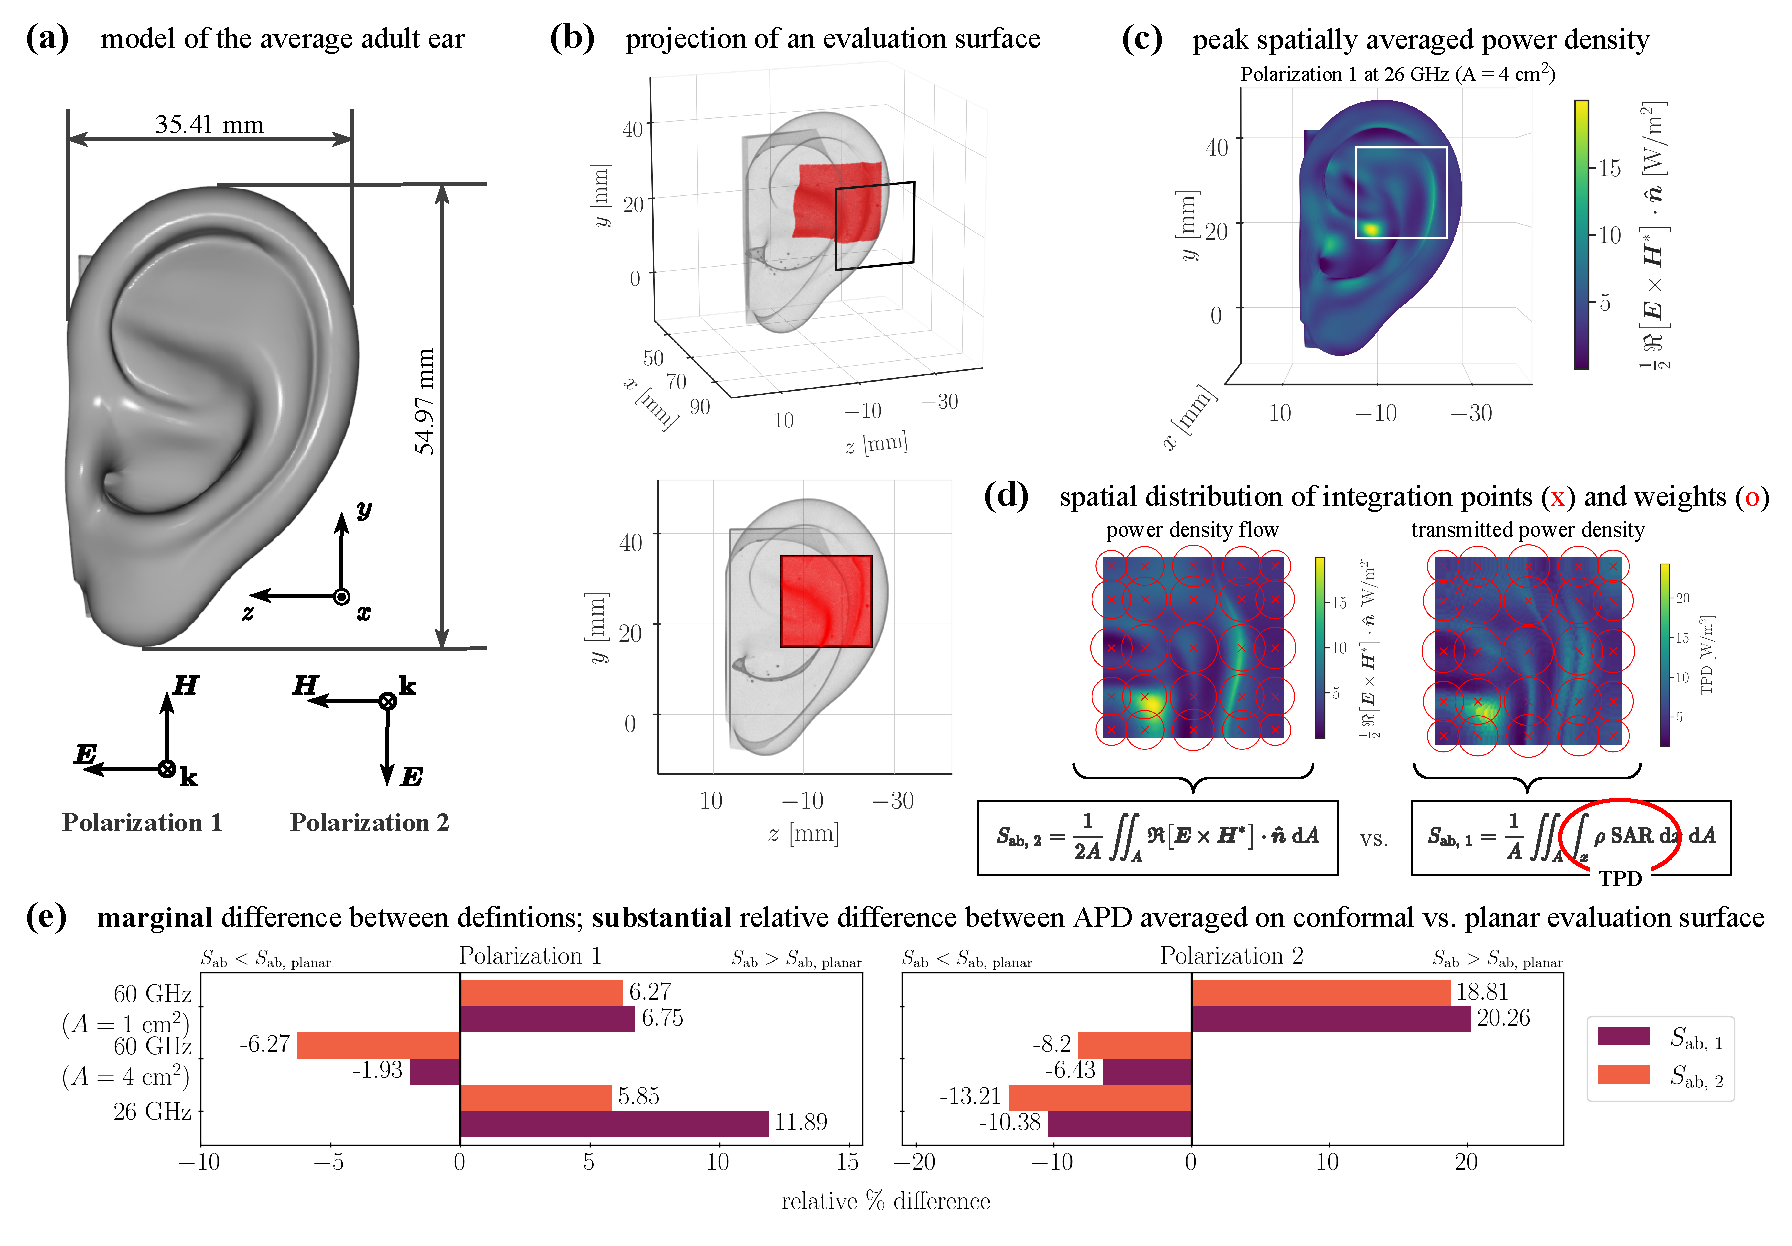
\includegraphics[width=\textwidth]{artwork/Kapetanovic2022JERM.pdf}
    \caption{Overview of the assessment process and quantitative comparison of the peak absorbed power density spatially averaged on the conformal evaluation surface of the average adult ear model by using the volumetric and surface definition.}
    \label{fig:Kapetanovic2022JERM}
    \end{center}
\end{figure}

The analysis presented in the study is focused on quantifying the superficial exposure of the human ear as it is among the most irradiated body parts in common exposure scenarios in terms of two different definitions of the spatially averaged \gls{apd} at \SIlist{26;60}{\GHz} -- frequencies upcoming for the \gls{5g} standard for broadband cellular networks.
The findings demonstrate a strong effect of irregularities in the geometry of the averaging surface, e.g., curvature (either convex or concave), sharp edges, deformities, etc., on the spatial distribution of \gls{em} power and the spatially averaged dosimetric quantities, whose accuracy is of utmost importance especially at \gls{mmw}.
It is shown that the spatially averaged \gls{apd} is up to \SI{20}{\percent} greater on conformal surfaces where morphological features of the average human ear are considered.
Additionally, it has been confirmed that only marginal differences (up to \SI{6}{\percent} relative difference) exist between the volumetric and surface definition of the spatially averaged \gls{apd}.
This is due to shallow depth of penetration of \gls{emf} into the tissue at considered frequencies (up to \SI{1}{\mm} at \SI{26}{\GHz} and only up to about \SI{0.5}{\mm} at \SI{90}{\GHz} assuming dielectric properties of dry skin~\cite{Sasaki2017Monte}).

\subsection{Author Contributions}
Authors: Ante Kapetanović, Giulia Sacco, Dragan Poljak and Maxim Zhadobov.\\
Conceptualization: AK, GS and MZ; data curation: AK and GS; formal analysis: AK and GS; funding acquisition: DP and MZ; investigation: AK; methodology: AK; project administration: AK, GS, DP and MZ; software: AK and GS; supervision: DP and MZ, validation: AK and GS; visualization: AK; writing -- original draft: AK and GS; writing -- review and editing: AK, GS, DP and MZ.

\subsection{Supplementary Materials}
Data and code are available on GitHub: \url{https://github.com/akapet00/EMF-exposure-analysis/tree/main/playground/IEEE-J-ERM_paper}.


\section{On the Applicability of Numerical Quadrature for Double Surface Integrals at 5G Frequencies}
\label{sec:publication_4}
\subsection{Abstract}
The human exposure assessment to wireless communications systems including the fifth generation (5G) mobile systems is related to determining the specific absorption rate (SAR) or the absorbed power density (APD).
The assessment of both quantities requires the use of various numerical techniques, including moments method (MoM).
As the use of MoM results in a fully populated system matrix, a tremendous computational cost is incurred, both in terms of matrix fill time and memory allocation, as the matrix size is directly related to frequency of the problem.
This paper investigates the applicability of numerical integration at frequencies related to 5G.
The novelty of this work is related to the comprehensive set of tests of various combination of source and observation triangles using the developed unit cube test.
A number of convergence tests were performed to investigate the effects of the increasing frequency and the discretization scheme on the numerical solution, as well as to determine how to curb the computational requirements by the proficient use of numerical integration.
The results show that in the lower gigahertz range, lower integration orders could be used, resulting in the decrease of matrix fill time without loss of solution accuracy.

\subsection{Impact Statement}
In all three previously outlined publications, surface integrals of the scalar and vector field have been approximated by using the \gls{2-d} $n$-degree Gauss-Legendre quadrature~\cite{Abramowitz1972Handbook} or the adaptive Gauss-Kronrod quadrature~\cite{Piessens1983Quadpack} depending on whether the integrands are ``well-behaved'' or not.
Since ``behavior'' in this sense is a vaguely defined term as there is no strict mathematical definition for it, please refer to~\cite{Weisstein2023Pathological} for further explanation.
However, in neither publication, the reasoning for the choice of the specific quadrature scheme have been provided.

As the exposure assessment and dosimetry analysis relies on the use of sophisticated computational methods that require the iterative approximation of double surface integrals, the number of which is directly proportional to the operating frequency dictating the resolution of the \gls{em} model, it is of utmost importance to avoid the use of the quadrature degree greater than necessary to avoid increased computational cost.
The method of moments is used in this paper, which, although accurate for integral equation-based \gls{em} formulations, require fully populated system matrix whose size is related to the frequency of the problem.
This leads to the tremendous computational costs by means of the matrix fill time and corresponding memory allocation~\cite{Poljak2018conformal}.

In this paper, which is the direct extension of~\cite{Cvetkovic2021Study}, the comprehensive set of convergence tests for quadrature related to double surface integrals at frequencies related to \gls{5g} is demonstrated.
Specifically, examination on various combination of source and observation triangles has been performed.
Computational results demonstrate that the numerical solution at frequencies in the higher gigahertz range require the use of high quadrature orders as well as finer discretization schemes, resulting in significantly increased requirements for matrix storage as well as matrix fill time.
On the other hand, at lower gigahertz range by using an appropriate discretization scheme, lower integration orders could be used thereby facilitating the decrease of matrix fill time without actually lowering the accuracy of the solution.

\subsection{Author Contributions}
Authors: Mario Cvetković, Dragan Poljak, Ante Kapetanović and Hrvoje Dodig.\\
Conceptualization: MC and DP; data curation: MC; formal analysis: MC; funding acquisition: not applicable; investigation: MC, AK and HD; methodology: MC; project administration: MC, DP, AK and HD; software: MC; supervision: DP, validation: MC and AK; visualization: MC; writing -- original draft: MC; writing -- review and editing: MC, DP, AK and HD.
